\chapter{Liquid Hydrogen target}
\begin{refsection}
{\itshape In this chapter the Charge EXchange reaction, a calibration for the liquid XEnon Calorimeter, will be discussed and an in-depth description of the associated Liquid Hydrogen Target is given. 
Data taking, analysis, performances, and the different modifications will be also discussed.
This target was designed in 2020 to overcome some limitations of the previous and in the last two years went through some heavy re-development.
This calibration is cardinal for the correct functioning of the key subdetector of the MEG II experiment. It  was one of the main tasks in my involvement in this experiment and it absorbed a sizable portion of my time and effort.}

\section{Charge EXchange reaction}
\section{BGO}

\section{2021}
    I started my Ph.D in November 2020 but I joined the activities after the first year, in October 2021. For this reason, I did not participate in the development of the first iteration of the target and I joined the first tests and data taking.

    \subsection{Data taking}
        \begin{figure}
            \centering
            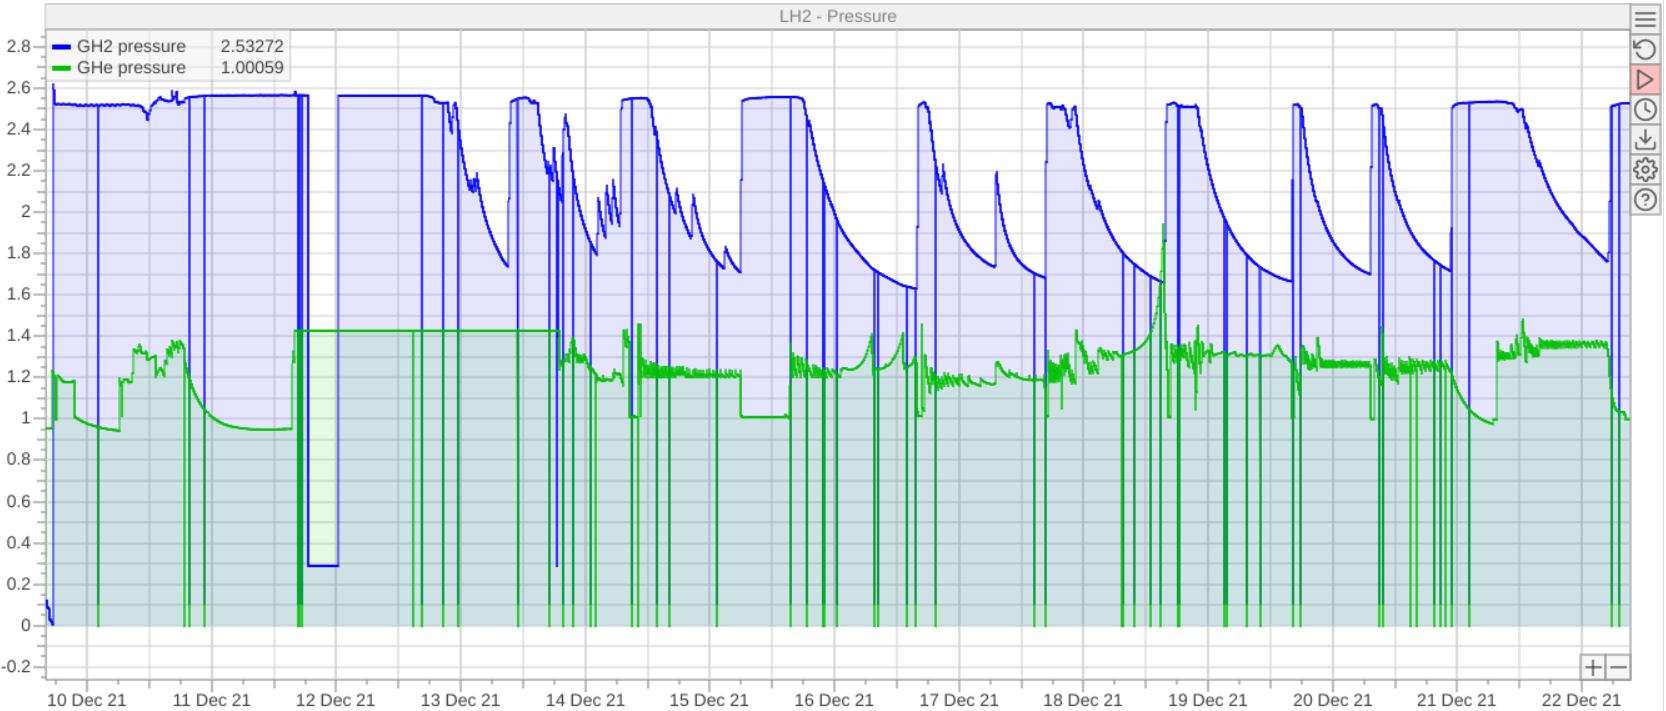
\includegraphics[width = \textwidth]{Figures/LH2/2021CEX_LH2.png}
            \caption{Measured hydrogen pressure in the target and helium pressure in the dewar used for cooling during 2021 CEX data taking. 
            Beam was ON when the target was considered `full enough': below AAA bar, meaning \SI{0}{\%}. 
            This translates to a time efficiency of $\varepsilon_{2021}\approx0$. 
            Unfortunately, the low efficiency prevented the collection of the necessary statistics for every patch of the XEC.}
            \label{fig:CEX2021}
        \end{figure}
    
    \subsection{Data anlaysis}
    \subsection{PM2022}
\section{2022}
    \subsection{Upgrades}
        \paragraph{He circuit}
        \paragraph{Cup}
        \paragraph{Shielding}
        
    \subsection{Data taking}
        \begin{figure}
            \centering
            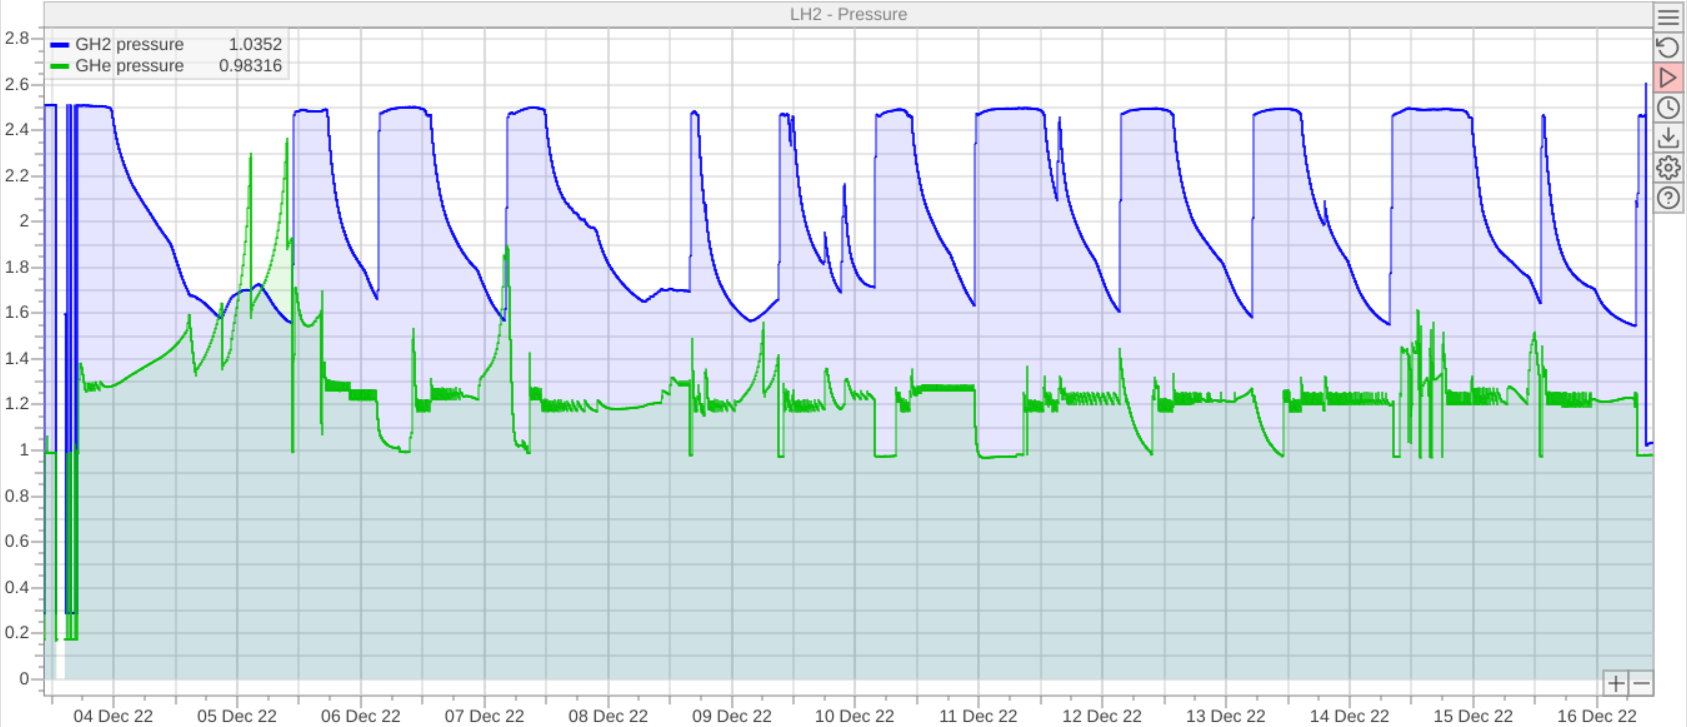
\includegraphics[width = \textwidth]{Figures/LH2/2022CEX_LH2.png}
            \caption{Measured hydrogen pressure in the target and helium pressure in the dewar used for cooling during 2022 CEX data taking. 
            Beam was ON when the target was considered `full enough': below AAA bar, meaning \SI{0}{\%}.  
            This translates to a time efficiency of $\varepsilon_{2022}\approx0$ (against $\varepsilon_{2021}\approx0$). 
            The improvement in efficiency allowed us to collect the necessary statistics for every patch of the XEC.}
            \label{fig:CEX2022}
        \end{figure}

    \subsection{Data analysis}

\section{2023}
    Although the 2022 CEX campaign was much more successful than the previous one, the limitations of this design and the second iteration dictated a hectic schedule during data taking. 
    The (somewhat risky) modification of the liquid hydrogen cup turned out to be a good improvement but there was still room for refinement. 
    For this reason, we went back to the drawing board.

    \subsection{Upgrades}
        \paragraph{He circuit}
        \paragraph{Cup}
        \paragraph{Shielding}
    \subsection{Data taking}
    \subsection{Data anlaysis}

\section{Conclusions}

\printbibliography[
    heading = bibliographychapter,
    title=Bibliography on \ce{LH2}
]

\end{refsection}
